\documentclass{beamer}
\usepackage{textpos}
\setlength{\TPHorizModule}{1cm} % Horizontale Einheit
\setlength{\TPVertModule}{1cm} % Vertikale Einheit
\usepackage{lmodern}
\usepackage{xcolor}
\usepackage{algpseudocode}
\usepackage{amsmath}
\usepackage{tcolorbox}
\usepackage{tikz}
\usepackage{fancyvrb}
\usepackage{soul}
\usepackage{tabularx, booktabs}
\newcolumntype{Y}{>{\centering\arraybackslash}X}
\usepackage[update,prepend]{epstopdf}
\usepackage{adjustbox}
\usepackage{setspace}
\usepackage[font={scriptsize}, justification=centering]{caption}
\usepackage[font={color=black}]{subcaption}
\usepackage{ellipsis}
\usetikzlibrary{decorations.pathmorphing,calc}
\usetikzlibrary{decorations.pathreplacing}
\usetikzlibrary{positioning}
\usepackage{chemarrow}
\usepackage{slashbox}
\usepackage[ruled,vlined,linesnumbered]{algorithm2e}
\usepackage{siunitx}
\usepackage{relsize}
\usepackage{3dplot}
\usepackage{threeparttable}
\usetikzlibrary{fit}
\usepackage[utf8]{inputenc}
\usepackage[upright]{fourier}
\usetikzlibrary{matrix,arrows,decorations.pathmorphing}
\usepackage{xparse}
\usepackage[nomessages]{fp}% http://ctan.org/pkg/fp
\usetikzlibrary{calc}
\usepackage{breqn} %for dmath
\usepackage{hyperref} 
\usepackage{arydshln}
\usetikzlibrary{shapes,fit}
\definecolor{univred}{rgb}{0.7, 0.0, 0.0}
\definecolor{drkgreen}{rgb}{0,0.26,0.15}
\definecolor{aureolin}{rgb}{0.99,0.93,0.0}
%
%
\newcolumntype{C}[1]{>{\centering\let\newline\\\arraybackslash\hspace{0pt}}m{#1}}
\setbeamertemplate{background canvas}{%
    {\color{univred}\noindent\makebox[\paperwidth]{\rule{\paperwidth}{2.5ex}}
}}
\setbeamertemplate{frametitle}{\color{black}\bfseries\vskip2ex\insertframetitle\par\vskip-6pt\hrulefill}
\addtobeamertemplate{frametitle}{}{%
%CMU logo in header
    \begin{textblock*}{100mm}(0.87\textwidth,-1.425cm)
        \includegraphics[height=1.5cm,width=1.9cm,keepaspectratio]{cm_logo}
    \end{textblock*}
%ECE logo in footer
    \begin{textblock*}{10mm}(-.8cm,7.5cm)
        \includegraphics[height=2cm,width=2.5cm,keepaspectratio]{ece}
    \end{textblock*}
}
\addtobeamertemplate{footnote}{}{\vspace{2ex}}
\setbeamercolor*{item}{fg=black}
\setbeamertemplate{footline}[page number]{}
\setbeamercolor{page number in head/foot}{fg=univred}

\makeatletter
\newcommand{\defhighlighter}[3][]{%
    \tikzset{every highlighter/.style={color=#2, fill opacity=#3, #1}}%
}

\defhighlighter{yellow}{.5}
\newcommand{\highlight@DoHighlight}{
    \fill [ decoration = {segment length=13pt}
        , outer sep = -15pt, inner sep = 0pt, decorate
    , every highlighter, this highlighter ]
    ($(begin highlight)+(0,8pt)$) rectangle ($(end highlight)+(0,-1pt)$) ;
}

\newcommand{\highlight@BeginHighlight}{
    \coordinate (begin highlight) at (0,0) ;
}

\newcommand{\highlight@EndHighlight}{
    \coordinate (end highlight) at (0,0) ;
}

\newdimen\highlight@previous
\newdimen\highlight@current

\DeclareRobustCommand*\highlight[1][]{%
    \tikzset{this highlighter/.style={#1}}%
    \SOUL@setup
  %
    \def\SOUL@preamble{%
        \begin{tikzpicture}[overlay, remember picture]
            \highlight@BeginHighlight
            \highlight@EndHighlight
        \end{tikzpicture}%
    }%
  %
    \def\SOUL@postamble{%
        \begin{tikzpicture}[overlay, remember picture]
            \highlight@EndHighlight
            \highlight@DoHighlight
        \end{tikzpicture}%
    }%
  %
    \def\SOUL@everyhyphen{%
        \discretionary{%
            \SOUL@setkern\SOUL@hyphkern
            \SOUL@sethyphenchar
            \tikz[overlay, remember picture] \highlight@EndHighlight ;%
        }{%
        }{%
            \SOUL@setkern\SOUL@charkern
        }%
    }%
  %
    \def\SOUL@everyexhyphen##1{%
        \SOUL@setkern\SOUL@hyphkern
        \hbox{##1}%
        \discretionary{%
            \tikz[overlay, remember picture] \highlight@EndHighlight ;%
        }{%
        }{%
            \SOUL@setkern\SOUL@charkern
        }%
    }%
  %
    \def\SOUL@everysyllable{%
        \begin{tikzpicture}[overlay, remember picture]
            \path let \p0 = (begin highlight), \p1 = (0,0) in \pgfextra
            \global\highlight@previous=\y0
            \global\highlight@current =\y1
        \endpgfextra (0,0) ;
        \ifdim\highlight@current < \highlight@previous
        \highlight@DoHighlight
        \highlight@BeginHighlight
        \fi
    \end{tikzpicture}%
    \the\SOUL@syllable
    \tikz[overlay, remember picture] \highlight@EndHighlight ;%
}%
\SOUL@
}
\makeatother

\title{\color{univred} A Comparison of Antenna Placement Algorithms}
\author{Abhinav Jauhri}
\date{\today}
\begin{document}
\begin{frame}
    \color{univred}
    \titlepage
    \begin{center}
        {\tiny Backup Slides}
\end{center}
\end{frame}

\begin{frame}[fragile]{Exhaustive Algorithm}
    Pseudo code: 
    \vspace*{0.5cm}
    \begin{Verbatim}[fontsize=\tiny]
    def exhaustive_search::initialize: 
        makeConfigurations(new antenna_configuration,0) 

    def make_configurations(configuration, count): 
        if configuration.length == selected_antennas.length: 
            population.push_back(configuration)
            return 

        for i in range(0,selected_antennas[count].points.size()):
            if not selected_antennas[count].points.at(i) in configuration: 
                configuration.push_back(selected_antennas[count].points.at(i))
                make_configurations(configuration,count+1)
                configuration.pop_back();
    \end{Verbatim}
\end{frame}


\begin{frame}{Parameter Selection - GA}
 \begin{figure}
\centering
\vspace*{-0.4cm}
    \includegraphics[scale=0.48]{../paper/FIG/ga_mut}%
\end{figure}
\end{frame}

\begin{frame}{Parameters - GA and ES}
        Genetic Algorithm
    \adjustbox{max width=\columnwidth}{\tiny
        \begin{tabularx}{\columnwidth}{c *{6}{Y}}
            \toprule
            Test Case & Population & Generations & Mutation Prob. & Crossover Prob. & Elitism & Tournament Size \\
            \midrule
            tc1 & 500 & 10 & 0.1 & 0.6 & 50 & 50 \\
            tc2 & 3600 & 10 & 0.1 & 0.6 & 360 & 360 \\
            tc3 & 8500 & 10 & 0.1 & 0.6 & 850 & 850 \\
            tc4 & 1500 & 10 & 0.1 & 0.6 & 150 & 150 \\
            \bottomrule
        \end{tabularx}
    }\\
    \vspace*{1cm}
Evolutionary Strategy
 \adjustbox{max width=\columnwidth}{\tiny
        \begin{tabularx}{\columnwidth}{c *{4}{Y}}
            \toprule
            Test Case & $\mu$ & $\lambda$ & Generations\\
            \midrule
            tc1 & 70 & 490 & 10  \\
            tc2 & 550 & 3850 & 10  \\
            tc3 & 1200 & 8400 & 10 \\
            tc4 & 220 & 1540 & 10 \\
            \bottomrule
        \end{tabularx}
    } 
    {\tiny $1/7$ ratio between and $\mu$ and $\lambda$\footnotemark. Higher ratios led to  higher evaluations per run \break
    [1] Eiben, A. E., \& Smith, J. E. (2003). Introduction to evolutionary computing.}
\end{frame}

\begin{frame}[t]{Parameters - SA}
    \begin{enumerate}
        \item Initial Temperature $\in [0.23, 0.27]$ 
        \item Cooling Schedule: Geometric cooling $T_{i+1} = \tau T_{i}~ (\alpha < 1)$ where $\tau \in [0.99, 1)$ such that $T_i <= 10^{-4}$ at $50\%$ iterations
    \end{enumerate}
\end{frame}

\begin{frame}{Parameter Selection - SA (todo)}
\end{frame}


\begin{frame}{Test Cases - Contour Plots}
    \begin{columns}
        \begin{column}{.5\columnwidth}
            \begin{figure}
                    \vspace*{-.8cm}
                \begin{subfigure}{\columnwidth}
                    \centering
                    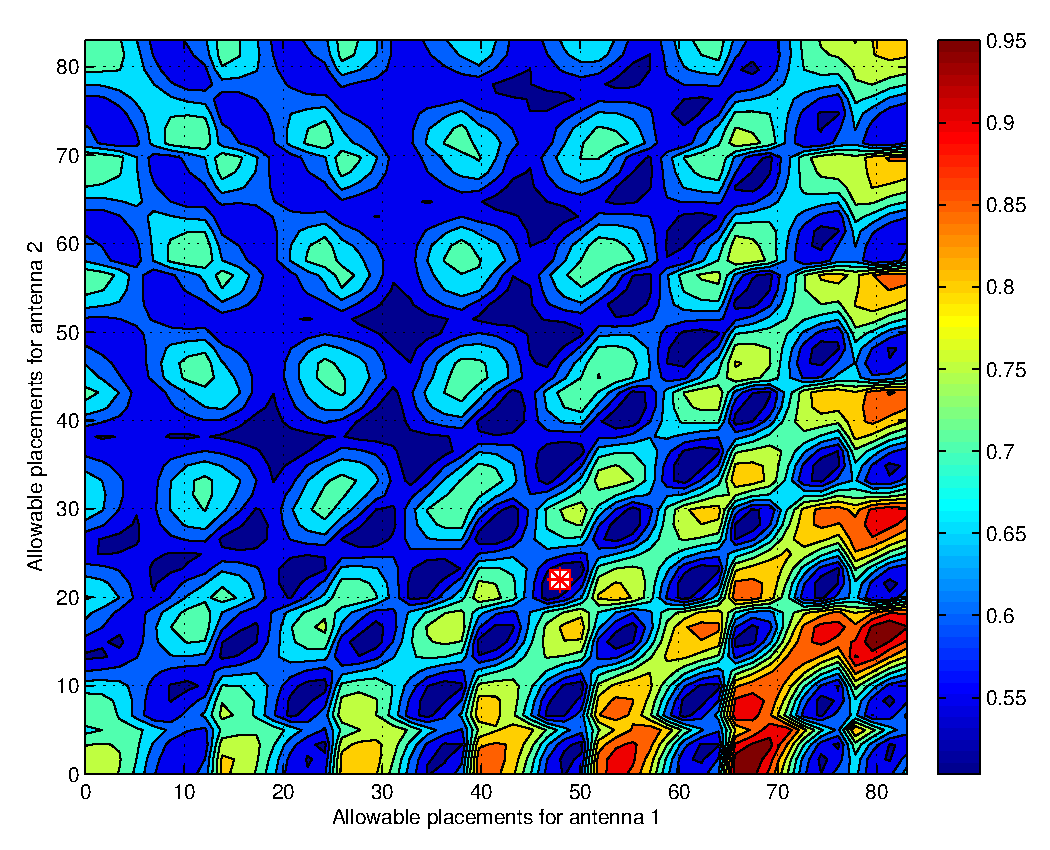
\includegraphics[trim=5 0 10 0, clip,scale=0.23]{../paper/FIG/tc1_contour}%
                \vspace*{-0.2cm}
                    \caption*{\tiny Test Case \#1}
                \end{subfigure}\hfill\\
                \begin{subfigure}{\columnwidth}
                    \centering
                    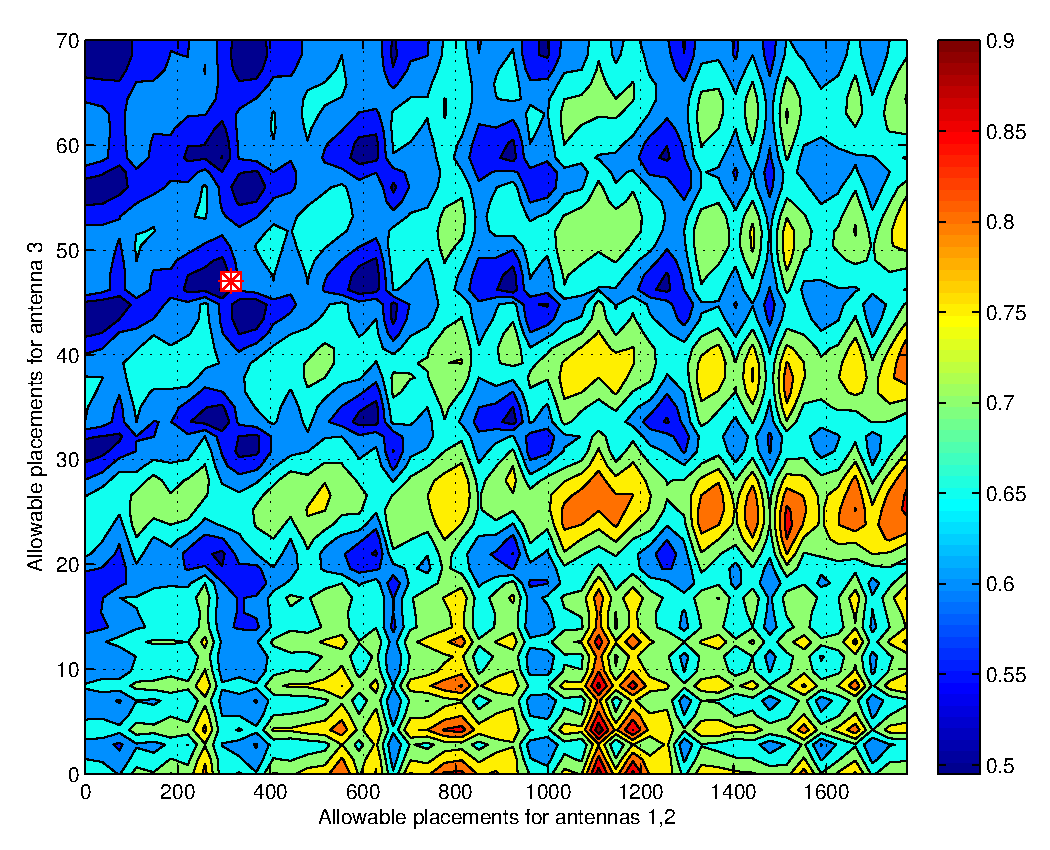
\includegraphics[trim=5 0 10 0, clip,scale=0.23]{../paper/FIG/tc3_contour}%
                    \vspace*{-0.2cm}
                    \caption*{\tiny Test Case \#3}%
                \end{subfigure}\hfill%
            \end{figure}
        \end{column}
        \begin{column}{.5\columnwidth}
    \begin{figure}
                    \vspace*{-.8cm}
                \begin{subfigure}{\columnwidth}
                    \centering
                    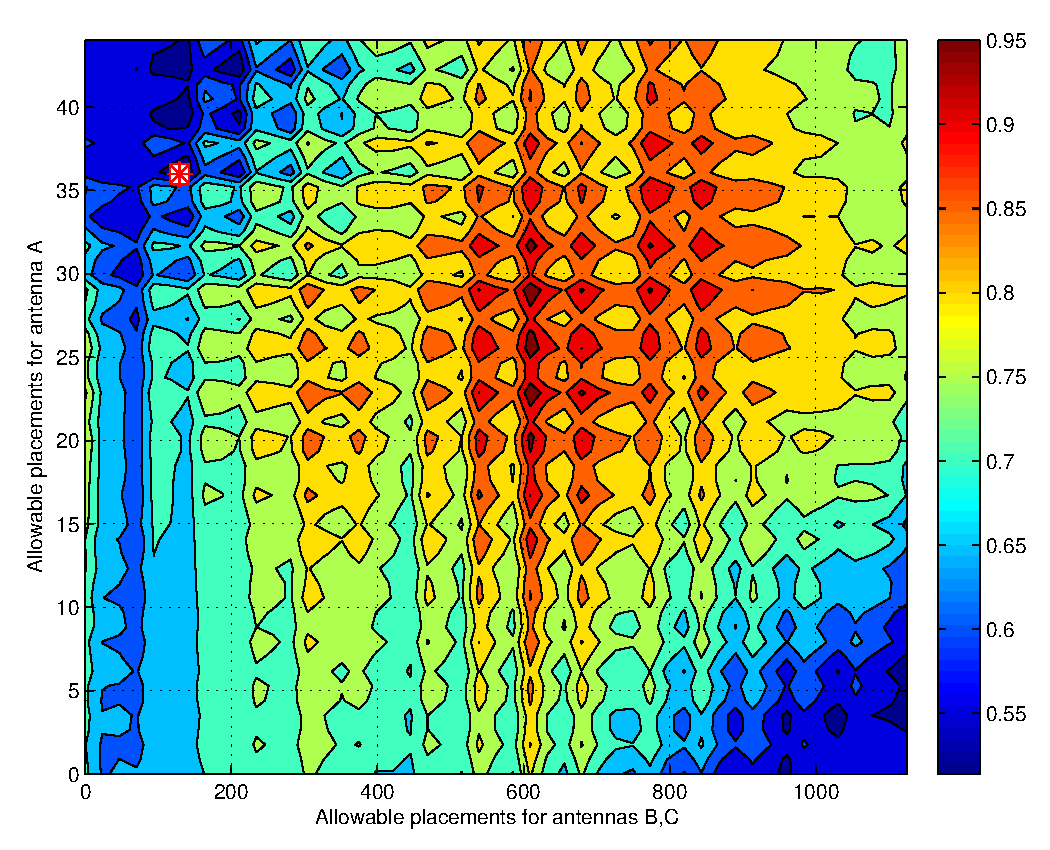
\includegraphics[trim=5 0 10 0, clip,scale=0.23]{../paper/FIG/tc2_contour}%
                \vspace*{-0.2cm}
                    \caption*{\tiny Test Case \#2}
                \end{subfigure}\hfill\\
                \begin{subfigure}{\columnwidth}
                    \centering
                    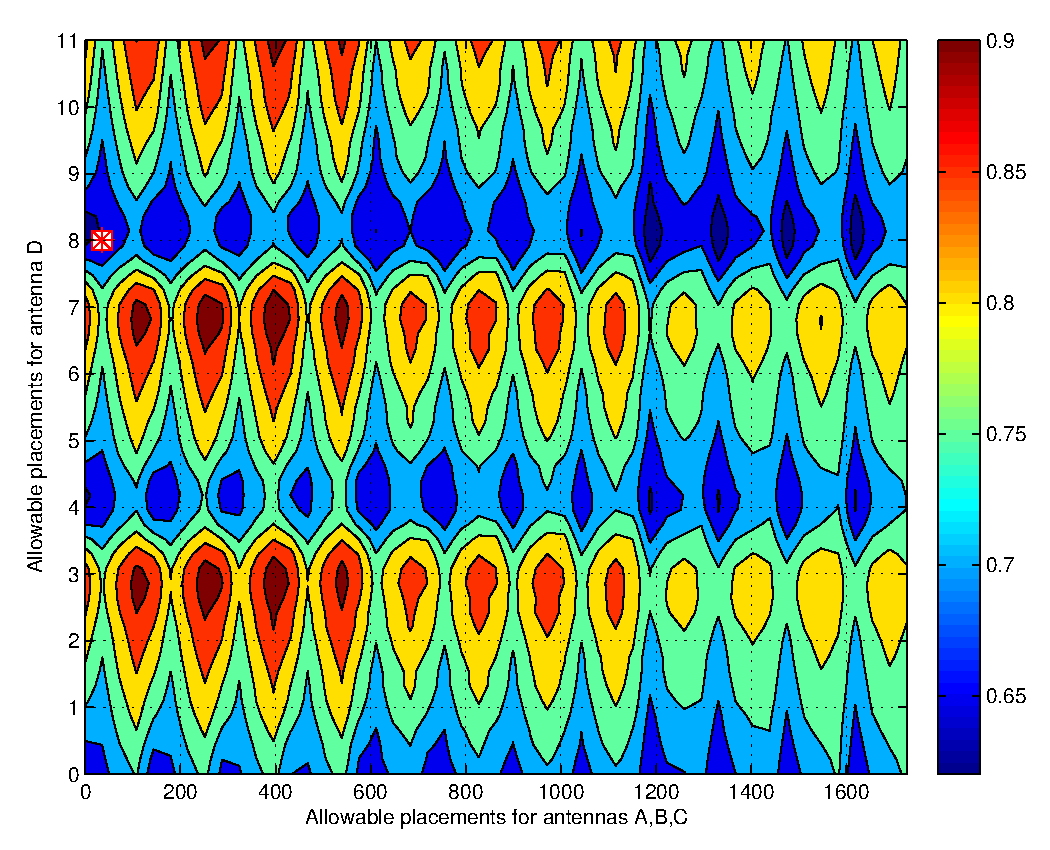
\includegraphics[trim=5 0 10 0, clip,scale=0.23]{../paper/FIG/tc4_contour}%
                    \vspace*{-0.2cm}
                    \caption*{\tiny Test Case \#4}%
                \end{subfigure}\hfill%
            \end{figure}

        \end{column}
    \end{columns}
\end{frame}


\begin{frame}{Search space for larger problem}
 \begin{figure}
     \vspace*{-.2cm}
\centering
    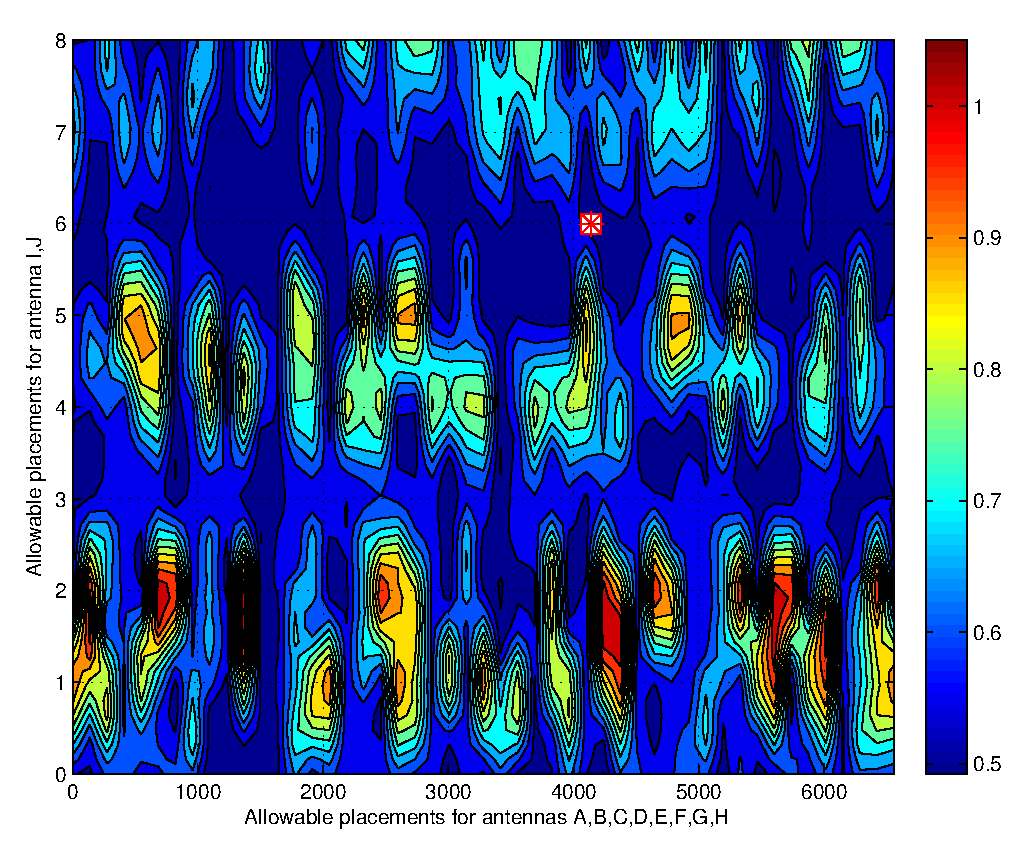
\includegraphics[scale=0.5]{../paper/FIG/tc5_contour}%
    \vspace*{-.1cm}
     \caption*{\tiny Search space for problem with $10$ antennas resembles contours as seen in experiments}
\end{figure}
\end{frame}

\begin{frame}{Results - Test Case 5}
    \begin{columns}
        \begin{column}{\columnwidth}
            {\tiny Sample size = 1000}
            \adjustbox{max width=\columnwidth}{\tiny
                \begin{tabularx}{\columnwidth}{@{}l *4{>{\centering\arraybackslash}X}@{}} 
                    \toprule
                    Algorithm
                    & \multicolumn{2}{c}{\%Evaluations vs. Exhaustive}  
                    & \multicolumn{2}{c}{Best fitness}\\
                    \cmidrule(lr){2-3} \cmidrule(l){4-5}
                    & Mean & Std. Dev. &  Mean & Std. Dev. \\
                    \midrule
ES & 15.11 & 7.10 & 0.49975 & 0.00000 \\
SA & 11.58 & 3.50 & 0.49975 & 0.00000 \\
GA & 34.08 & 15.57 & 0.49977 & 0.00012 \\
HC & 0.13 & 0.08 & 0.50407 & 0.00761 \\
                    \bottomrule
                \end{tabularx}
            } \vspace*{-0.35cm}
            \begin{figure}
                \centering
                    \includegraphics[trim=0 10 0 30,clip,height=5cm,width=8cm]{../paper/FIG/tc5_mf}%
            \end{figure}
        \end{column}
    \end{columns}
\end{frame}


\begin{frame}{Equivalence of fitness to efficiency}
    \small For a particular test case, fitness change of $0.001$ is equivalent to either the corresponding value under expected gain ($\mathbb E_{\Delta g}$) column, or difference in coupling ($\Delta_c$).
    \begin{table}
        \centering
        \begin{threeparttable}
            \begin{tabular}{|C{1cm}|C{2.5cm}|C{2.5cm}|} \hline
                ID& $\mathbb E_{\Delta g}$ (dB) & $\Delta_{c}$ (dB) \\ \hline
                tc1 & 9.34 & 0.055 \\ \hline
                tc2 & 9.28 & 0.13 \\ \hline
                tc3 & 9.28 & 0.15 \\ \hline
                tc4 & 9.33 & 0.057 \\
                \hline\end{tabular}
        \end{threeparttable}
    \end{table}
\end{frame}

\begin{frame}{Differential Evolution}
    \begin{enumerate}
        \item [Step 1:] Randomly initialize a population 
        \item [Step 2:] Mutation: For each target $x_i^g, i \in \{1, 2, 3 \ldots, NP\}$, a mutant vector is formed for the subsequent generation using:
            \[v_i^{g} = x_{r_1}^g + F \cdot (x_{r_2}^g - x_{r_3}^g), \]
            where $F \in [0,2]$ and $r_1, r_2, r_3$ are mutually different and also $ \neq i$
        \item [Step 3:] Recombination: Formulate a trial vector as:
    \[u_i^{g+1} = 
        \begin{cases}
            v_{ij}^g, & \text{if rand()} \leq CR \text{ or }j = \textit{rnbr(i)} \\
            x_{ij}^g, & \text{if rand()} > CR \text{ and }j \neq \textit{rnbr(i)} \\
    \end{cases}\]
        \item [Step 4:] Selection: Compare trial vector $u_i^{g+1}$ and target vector $x_i^g$, and select the vector which yields a smaller cost function.\\
        \item [Step 5:] Termination check
    \end{enumerate}
\end{frame}


\begin{frame}{Particle Swarm Optimization}
    \begin{enumerate}
        \item [Step 1:] Randomly initialize velocity and position of all particles
        \item [Step 2:] At each iteration, updated velocity as follows:
            \[ v_i = wv_i + c_1 R_1 (p_{i,best} - p_i) + c_2 R_2 (g_{best} - p_i) ,\]
            where $p_{i,best}, g_{best}$ are positions with best objective value found so far by particle and entire population respectively, $c_1,c_2$ are weighting factors, $R_1,R_2 \thicksim \mathbb U(0,1)$, $w$ is parameter cooling
        \item [Step 3:] Position updating
            \[ p_i = p_i + v_i \]
        \item [Step 4:] Memory updating: Update $p_{i,best}$ and $g_{best}$
        \item [Step 5:] Termination check
    \end{enumerate}
\end{frame}

\end{document}
